\subsubsection{Schema DSP}
\label{sec:Schema_DSP}

In diesem Abschnitt wird die Beschaltung des STM32F412 beschrieben. Für die genaue Pinkonfiguration, Pinfunktionen und Konfiguration dient das \\
Kapitel \ref{sec:CubeMX} "Konfiguration mit STM32CubeMX".

\paragraph{I2S Schnittstelle}

Die Hersteller des TLV320 und des STM32 verwenden nicht die gleichen Signalbezeichnungen für das Pinout der Bauteile.
Die Tabelle \ref{tab:I2SPins} stellt den Bezug der Signale an beiden Chips her und zeigt die Signalrichtung und Verbindung wie sie im Schema des DSP Boards zur Anwendung kommt.

\begin{table}[H]
	\centering
	\begin{tabular}{|l|l|c|l|l|}
	\hline
	\textbf{STM32} & \textbf{Signal} & \textbf{Richtung}         & \textbf{Signal} & \textbf{TLV320} \\ \hline
	PC2            & MISO            & $\leftarrow$  & DOUT            & 6               \\ \hline
	PC3            & MOSI            & $\rightarrow$ & DIN             & 4               \\ \hline
	PB12           & WS              & $\rightarrow$ & LRCIN           & 5               \\ \hline
	PB12           & WS              & $\leftarrow$  & LRCOUT          & 7               \\ \hline
	PA2            & CKIN            & $\leftarrow$  & CLKOUT          & 2               \\ \hline
	\end{tabular}
	\caption{Signale zwischen dem DSP und dem Codec}
	\label{tab:I2SPins}
\end{table}


\paragraph{Bootloader und Bootpins}

Die STM32 Familie hat einen integrierten Firmware upgrade Bootloader.
Um diesen zu aktivieren müssen die externen BOOT[1:0] Pins im richtigen Muster gesetzt werden.
In diesem Projekt wird die Firmware über den USB mini-B Connector auf den STM32 überspielt.
Das Application Note AN2606 \cite[p.136]{AN2606} beschreibt die Pinkonfiguration für diesen Anwendungsfall.
So muss kein Pull-Up Widerstand an der \texttt{USB\_DP} Leitung angeschlossen sein um die OTG-Bedingungen zu erfüllen.
Ausserdem muss eine externe Clock mit einer Frequenz zwischen $4\si{MHz}$ und $26\si{MHz}$ verfügbar sein, was durch den externen Quartz \textit{Y1} erreicht wird.

Die Bootpins müssen gemäss der Application Note AN2606 \cite[Table 2]{AN2606} mit dem Boot Pattern 1 gesetzt werden um den DFU Bootloader zu starten.
Unten in der Tabelle sind die beiden Boot Modi zusammengefasst.

Der BOOT1 Pin ist beim STM32F412 auf PB2.

\begin{table}[H]
\centering
\begin{tabular}{|l|c|c|}
\hline
\textbf{Boot Mode} & \textbf{BOOT1} & \textbf{BOOT0} \\ \hline
Bootloader         & 0              & 1              \\ \hline
Normal             & 0              & 0              \\ \hline
\end{tabular}
\caption{Mode Auswahl über BOOT[1:0] Pins}
\end{table}

\paragraph{Bootstrap Schaltung für Bootpin}

Der STM32 ist fähig, per Software in den Bootloader Modus zu wechseln \cite{STM32-Softreset-Stackoverflow}. Die Software dazu ist jedoch aufwändiger als den Bootvorgang per Hardware auszulösen.

Aus diesem Grund ist der \texttt{BOOT0} Pin mit einem GPIO Pin (\texttt{PD2}) verbunden, Abbildung \ref{fig:Schema_Bootpin_Bootstrap}.

\begin{figure} [H]
	\begin{center}
		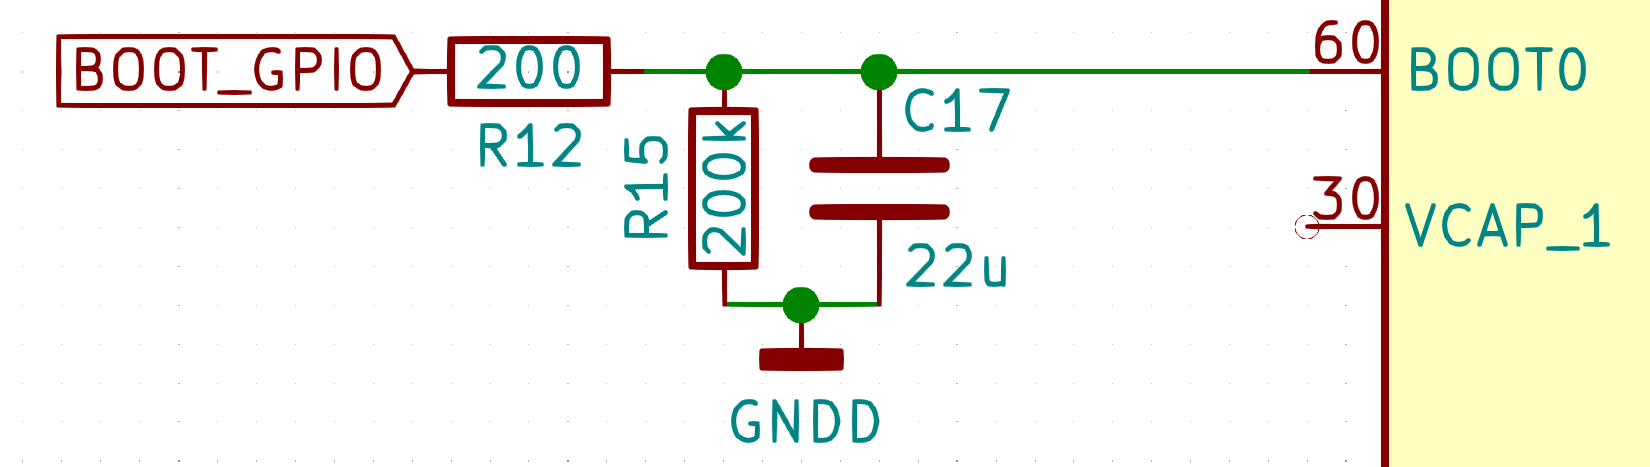
\includegraphics[scale=0.5]{../graphics/Schema_Bootpin_Bootstrap}
		\caption{Beschaltung des \texttt{BOOT0} Pins um über einen GPIO den Bootmodus zu setzen}
		\label{fig:Schema_Bootpin_Bootstrap}
	\end{center}
\end{figure}

So kann per Software der GPIO \texttt{PD2} auf \texttt{HIGH} gezogen werden und ein Software-Reset ausgelöst werden (siehe Abschnitt \ref{sec:Enter_DFU} in der Software), damit der STM32 im DFU-Bootloader startet.
Um dem Controller genügend Zeit zum Booten zu verschaffen, ist der \texttt{BOOT0} Pin mit einem $22\si{\mu F}$ Kondensator abgestützt. Der maximale Ausgangsstrom für einen GPIO beträgt $I_{GPIO}=25\si{mA}$ \cite[Table 14]{STM32f412}.
Mit dem Widerstand \textit{R12} beträgt der maximale Strom bei ungeladenem Kondensator \textit{C17}: 

\begin{equation}
I_{GPIO_{max}}=\frac{V_{CC}}{R_{12}}=\frac{3.3\si{V}}{200\si{\Omega}}=16.5\si{mA}
\end{equation}

Der Kondensator \textit{C17} wird über \textit{R15} entladen. Dabei bleibt dem STM32 ungefähr $1\tau=R*C$ Zeit um zu rebooten und den korrekten Pin-Zustand einzulesen. Diese Zeit beträgt ungefähr:

\begin{equation}
t_{reboot_{max}} \approx \tau = R_{15}*C_{17} = 200\si{k\Omega}*22\si{\mu F}=220\si{ms}
\end{equation}


\paragraph{Rotary Encoder und Buttons}

Einige Timer des STM32 unterstützen einen Encoder Modus, bei dem zwei GPIO Inputs zum Zählen der Encoderpulse verwendet werden können.

Alle 4 Pushbuttons sind an interruptfähige (EXTI) GPIO Pins angeschlossen. 
Die STM32 Familie unterstützt externe GPIO Interrupts an allen Pins. 
Dabei stehen 16 Interrupt Channels zur Verfügung, von welchen die Channel Nummer jeweils mit der GPIO Port Nummer übereinstimmen muss. 
Wie in der nachfolgenden Tabelle \ref{tab:EXTIPins} aufgeführt, werden insgesamt 4 EXTI Channels belegt.

\begin{table}[H]
	\centering
	\begin{tabular}{|l|l|r|}
	\hline
	\textbf{Signal}  & \textbf{GPIO} & \textbf{EXTI} \\ \hline
	Encoder 1 Button & PC12          & 12            \\ \hline
	Encoder 2 Button & PB13          & 13            \\ \hline
	Button 1         & PA0           & 0             \\ \hline
	Button 2         & PA1           & 1             \\ \hline
	\end{tabular}
	\caption{GPIO Mapping auf EXTI Interrupt Channels}
	\label{tab:EXTIPins}
\end{table}

\todo{SB: Jack Connector haben auch Interrupt}



